\documentclass[11pt]{article}
\usepackage[margin=0.8in]{geometry}\usepackage{graphicx}\usepackage[T1]{fontenc}\usepackage{hyperref}\setlength{\parskip}{6pt}\setlength{\parindent}{0pt}
\begin{document}
\begin{center}{\Large Finite-difference sieve: independent component review}\\2026-11-03 \quad T-1511\end{center}
\textbf{Result.} Accepted at component scope: 6,410 exact original/candidate sieve pairs passed; 21 named Lean declarations passed fresh axiom readback. Exact producer commit \texttt{c8db18e2c5} was published before candidate access and replay. This review preserves the distinction between an extracted component and its full producer integration.
\begin{center}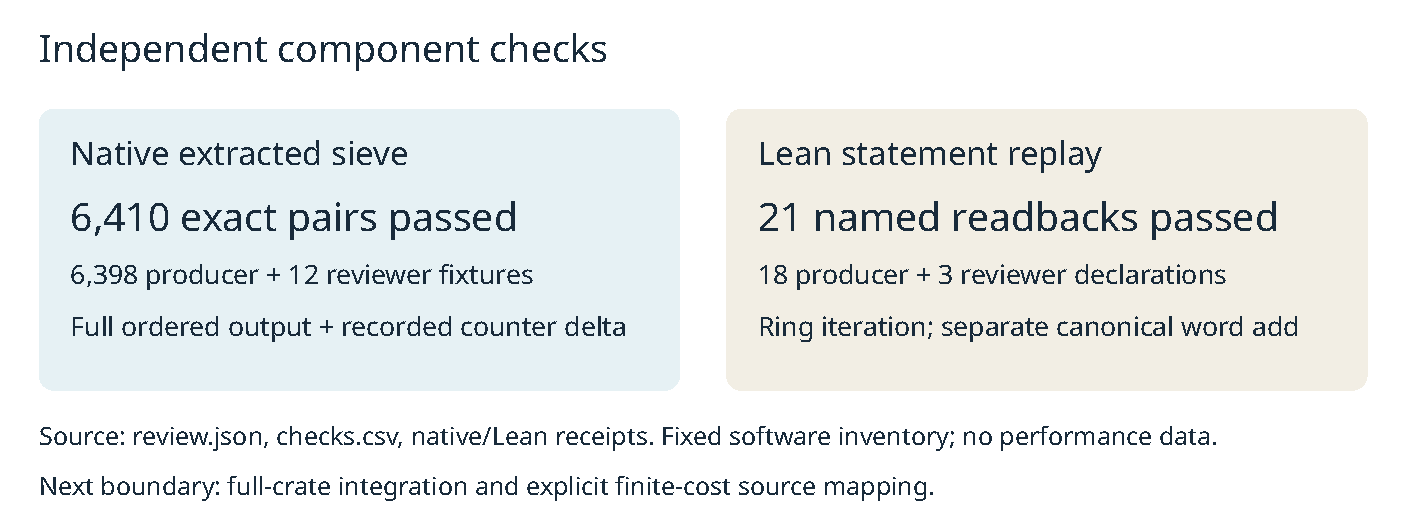
\includegraphics[width=\linewidth]{diagram.pdf}\end{center}
\textbf{Native checks.} The original 6,398 fixtures and 12 reviewer fixtures compare every returned scalar, candidate set and ordered bucket vector. Producer checks cover 20,207 recurrence sequences, 134,067 values, 32 boundary transitions and three deliberately wrong recurrences. Reviewer fixtures hit all five ordinary/exceptional branches; wrong counter and bucket outputs were rejected. Caught assertion diagnostics are retained.

\textbf{Source fidelity.} Fourteen native function bodies were compared exactly, including arithmetic, polynomial helpers, complement and original sieve. Real meter and tracked-set bytes match. The adaptation removes only the arithmetic counter serialization derive and supplies a plain Divisor field wrapper. It does not validate curve construction. Candidate captures current values then updates before either continue, preserving point order and ignoring inactive coefficient tails.

\textbf{Bounds and receipts.} One native attempt used a 120-second outer bound and 2-GiB address-space limit; one Lean attempt used 300 seconds and 8 GiB with one worker and declared heap/stack limits. Both passed; source inputs stayed unchanged. Execution durations are software validation overhead, not algorithm performance measurements. No collector or scientific trajectory ran.
\newpage
\section*{Counter statement and proof boundary}
Let $d$ be active degree and $k=2d+1$. The candidate deliberately performs the final unused recurrence update. The checked source-delta equations are:
\[
 M_{new}=M_{old}-kp,\qquad
 A_{new}=A_{old}+3p+2-kp,
\]
\[
 visits_{new}=visits_{old}-k(p-1).
\]
All other recorded arithmetic and meter fields agree in the paired checks. These describe the actual instrumentation, not every machine instruction. New Option/bounds machinery needs explicit classification under the finite source inventory before pricing admission. Scalar Copy follows the baseline coefficient-read convention.

\textbf{Lean scope.} The proof establishes recurrence and ordered fold over a commutative ring, plus a separate canonical UInt64 addition refinement with canonical operands and modulus at most $2^{63}$. It does not compose a whole iterative UInt64 or compiled Rust refinement. The native full sieve retains original prime/algebraic/complement preconditions. Reviewer controls cover a late ring step, inactive padding and overflow outside the bound. All 21 readbacks use only allowed axioms; the expected false theorem and three malformed inventories were rejected. A total of 28,797 dependency/toolchain files matched pre/post hashes.

\textbf{Independence.} Reviewer did not author the implementation or proofs, but proposed the recurrence direction and inspected the original sieve earlier. Advisory context is disclosed; this is not blind derivation. Shared dependency hash equality does not exclude transient concurrent changes.

\textbf{Limitations.} The reviewer bucket negative adds an element; no separate equal-cardinality permutation control ran. Exact ordered Vec comparison was inspected. The producer's earlier low-degree fixture failure remains in its published packet. This review does not admit scientific execution, whole-crate correctness, current full pricing or a performance gain.

\textbf{Reviewable artifacts.} \texttt{review.json}, \texttt{checks.csv}, extraction check, exact source snapshot, frozen wrappers, native/Lean receipts and named axiom list accompany the PDF. The large replay archive retains raw output, binaries, private proof artifacts and full input inventories with durable custody/readback. Candidate hash begins \texttt{01f98400}; proof hash begins \texttt{d475d7f1}. Historical data and producer sources are unchanged.
\end{document}
